\paragraph{Rivelatore di media}
Il seguente rivelatore si ottiene aggiungendo al rivelatore di QuasiPicco 
un filtro passa-basso.

\begin{figure}[h] %rivelatore di media
\centering
 \begin{circuitikz}[american voltages]
 \draw
 (0,2) to [full diode,o-,v=$V_d$] (2,2)
       to [resistor,l=$R_c$] (4,2)
       to [capacitor,l=$C$] (4,0)
 (4,2) to [short] (6,2)   
 (6,2) to [resistor,l=$R_d$] (6,0)
 (6,2) to [resistor] (9,2)
       to [short, -o] (10,2)
 (9,0) to [variable capacitor] (9,2)      
 (0,0) to [short, o-o] (10,0)
 ;
 \draw
 (-0.5,2) to [open, v=$V_{\text{in}}$] (-0.5,0)
 (10.6,2) to [open, v^>=$V_{\text{out}}$] (10.6,0)
 ;
 \draw [dashed] (6.8,-0.3) rectangle (9.6,2.3);
 \end{circuitikz}
 \caption{Rivelatore di media}
\end{figure}

Al variare della capacità variabile presente nel
filtro passa-basso si seleziona la frequenza da analizzare.

%\section{Caratteristiche dei rivelatori}
Le caratteristiche dei rivelatori di QuasiPicco e Media sono riportate nella norma
CISPR 16-1 (EN55016), le informazioni riguardo il rivelatore di Picco sono meno
dettagliate.
Se i valori misurati dal rilevatore di picco e QuasiPicco
coincidono, si può affermare che l'inviluppo del segnale è costante, ossia il
segnale è a onda continua, anche il rilevatore di media indicherà lo stesso valore.

\begin{center} %tabella parametri cispr 16
 \begin{tabular}{|>{\centering}m{3cm}|>{\centering}m{3cm}|>{\centering}m{3cm}|m{3cm}<{\centering}|}
  \hline
  \multicolumn{4}{|c|}{Banda CISPR} \\
  \hline
  &Banda A $9\sim150$\si{\kilo\hertz} & Banda B $0.15\sim30$\si{\mega\hertz} & Banda C $+$ D $30\sim300\sim1000$ \si{\mega\hertz} \\ \hline
  Ampiezza di banda \SI{-6}{\decibel} [\si{\kilo\hertz}] & 0.20 & 9 & 120 \\ \hline
  Costante di \underline{carica} [\si{\milli\second}]   & 45   & 1 & 1 \\ \hline
  Costante di \underline{scarica} [\si{\milli\second}]  & 500  & 160 & 550 \\ \hline
  \rowcolor{yellow}
  Costante meccanica [\si{\milli\second}] & 160 & 160 & 100 \\ \hline
  Fattore di sovraccarico dei circuiti che precedono il rilevatore [\si{\decibel}] & 24  & 30  & 43.5 \\ \hline
  Fattore di sovraccarico tra l'amplificatore a valle e lo strumento indicatore [\si{\decibel}] &  6 &  12 & 6 \\ \hline
 \end{tabular}
\end{center}

Al di sopra della frequenza di \SI{30}{\mega\hertz} si considerano i disturbi
come radiati.

La costante meccanica è ciò che trasforma un segnale variabile
nel tempo in un segnale costante, ossia rappresenta la costante di tempo
di uno smorzatore meccanico equivalente. La somma di tutti e 3 i tempi 
permette di calcolare la costante di tempo dell'intero rilevatore 
affinché la misura sia corretta.

\paragraph{Filtro a frequenza intermedia}
La figura \ref{fig:filtro_IF} riporta la risposta del filtro a frequenza intermedia con ampiezza
di banda pari a \SI{120}{\kilo\hertz} centrato su una frequenza generica.
\begin{figure}[h]
\centering
 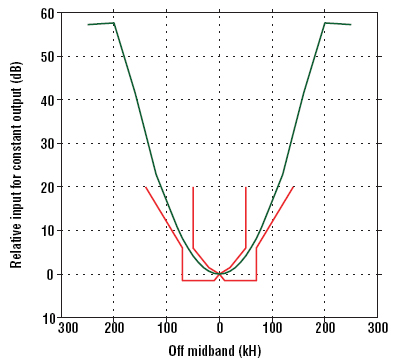
\includegraphics[width=0.6\linewidth]{IF_response}
 \caption{Risposta del filtro IF con ampiezza \SI{120}{\kilo\hertz} (banda \SI{30}{\mega\hertz} $\sim$ \SI{1}{\giga\hertz})}
 \label{fig:filtro_IF}
\end{figure}

L'asse verticale riporta \textit{l'ingresso relativo per un output costante}.
La maschera rossa è quella imposta dalla norma, la curva verde è solo
una possibile risposta del filtro, si può notare come la maschera
\textit{``stringa''} la curva alla frequenza di $\pm$ \SI{60}{\kilo\hertz}
per definire in maniera accurata la banda di \SI{120}{\kilo\hertz} a \SI{-6}{\decibel}.

Viene riportata la maschera fino a \SI{20}{\decibel} per verificare anche la selettività
del filtro, come si nota c'è un ampio margine lasciato al produttore del filtro.
Per permettere la realizzazione di filtri più selettivi, è consentita
una sovraelongazione fino a \SI{1.5}{\decibel} nell'intorno della frequenza centrale.

Il \textbf{rilevatore di media}, mediante il filtro passa-basso permette la rilevazione di componenti ad onda
continua in segnali a banda larga, ossia segnali sinusoidali puri.
